\documentclass[conference]{IEEEtran}
\IEEEoverridecommandlockouts
% The preceding line is only needed to identify funding in the first footnote. If that is unneeded, please comment it out.
\usepackage{cite}
\usepackage{amsmath,amssymb,amsfonts}
\usepackage{algorithmic}
\usepackage{graphicx}
\graphicspath{{images/}}
\usepackage{textcomp}
\usepackage{xcolor}
\def\BibTeX{{\rm B\kern-.05em{\sc i\kern-.025em b}\kern-.08em
    T\kern-.1667em\lower.7ex\hbox{E}\kern-.125emX}}
\begin{document}

\title{Bluetooth Low Energy (BLE) Implementation In Smart Home\\
}
\author{\IEEEauthorblockN{1\textsuperscript{st} Ammar Haziq Bin Mohd. Halim}
\IEEEauthorblockA{\textit{B. Eng. Electronic Engineering} \\
\textit{Hochschule Hamm-Lippstadt}\\
Lippstadt, Germany\\
ammar-haziq.bin-mohd-halim@stud.hshl.de}
\and
\IEEEauthorblockN{2\textsuperscript{nd} Muhammad Amjad Bin Abdul Malik}
\IEEEauthorblockA{\textit{B. Eng. Electronic Engineering} \\
\textit{Hochschule Hamm-Lippstadt}\\
Lippstadt, Germany \\
muhammad-amjad-bin.abdul-malik@stud.hshl.de}
\and
\IEEEauthorblockN{3\textsuperscript{rd}Muhammad Iqbal Bin Mohd. Fauzi}
\IEEEauthorblockA{\textit{B. Eng. Electronic Engineering} \\
\textit{Hochschule Hamm-Lippstadt}\\
City, Country \\
@stud.hshl.de}

}

\maketitle
\input{abstract}
\section{Introduction}
In apartments and houses, smart home refers to the employment of technical systems, automated procedures, and connected, remote-controlled gadgets. The functions' major goal is to increase the quality of life and ease of use in the house. Other objectives include improved security and energy efficiency thanks to connected, remote-controllable equipment. What distinguishes a smart house from a typical home? A smart house contains technologies that make our lives easier and more energy efficient. Today's technology includes smart home appliances, mobile devices, and home automation systems, all of which are increasingly networked.

It is human nature to find ways that make everyday life easier and more pleasant. The area of home automation in effect the predecessor of the smart home was brought to life through technological progress, in particular through the Internet and computer. Science fiction literature in the 1950s portrayed the first visions of homes that are monitored and controlled fully automatically by machines. The 1999 Disney film “Smart House” was about household computers and the consequences when smart machines take on a life of their own. And Disney proved to be unintentionally visionary in the part of the movie where the house’s intelligent control unit develops the feeling of jealousy. In reality, it will likely be a few years before machines can generate emotions, fortunately.
Scientists have already been working for more than 30 years on connecting home appliances and automating their use. Yet it’s only been in the past 15 years that the issue of the smart home has aroused broad public interest.
At its most basic, a smart home is one that uses so-called “smart” technology to automate and operate important tasks and devices, including lighting, heating and cooling, door locks for home security and not to forget fire alarms to increase home safety. Smart technology is technology that senses what is happening around a particular sensor or device and acts autonomously based on the information it collects. For example, a smart device might sense someone walking into a room and open the shades or turn off the lights or turn up the heat or whatever we have programmed it to do. The goal with these devices is to make your home “smart” enough that we are not bothered by manually performing mundane operations. In this thesis, we focus on prediction models in the smart home and their applications in designing various smart home services. We specifically focus on this category of prediction models and adopt a sequential prediction technique based on text compression algorithms for predicting the occupancy and mobility of the smart home residents. To evaluate the performance of the proposed solutions, a flexible small-scale smart home is constructed using motion sensors and a microcontroller. Several movement scenarios are designed, and the data has been collected by programming the microcontroller and the physical components.
For decades now, a wide range of different home appliances have helped make everyday life more pleasant, speed up processes and hence save time and work. So, what additional benefits does our smart home project deliver? Without the smart home, the impetus for a machine’s every action has to come from humans, who start processes manually and activate each device individually at the right time. The smart home relieves them of this work by enabling components to communicate with each other.

\section{Ease Of Use}
\subsection{Problem Statement}
One of the most obvious energy-wasting habits is leaving the lights on, and it’s also one of the easiest habits to fix. By simply turning off the lights when you leave a room or your home, you will save electricity and help your light bulbs last longer. If you think you might forget, use a smart home system to remotely monitor your lighting from your smartphone.

One of the four major old age problems include physical problems. Old age is a unique life phase characterized by various health, cognitive, emotional, social, and financial changes. Most people consider old age a problem-ridden stage of life, with aging problems usually occurring after 65. Physical decline and illness are one of the biggest problems aging people experience. Deteriorating health may prevent a person from doing things you enjoy or interfere with their routine activities. Also, chronic illness in the elderly may limit or cause a loss of independence, which is distressing for most people. 

\subsection{Smart Home Solution}
A smart home system is intended to solve a variety of issues. The main reason we created this project is that we want to make life easier and more comfortable inside our own home by making all of the systems in the house controllable with a single touch of a phone. All of the systems will be Bluetooth-connected, and we will be able to access them through specific apps. This project is also very effective in assisting elderly people and people with disabilities who have difficulty reaching certain switches in their homes. For example, a person in a wheelchair who is unable to walk would find it difficult to get up and turn on or off the light. With this project, they can easily control the lamp with their phone via Bluetooth. Furthermore, with the advent of smart heating and cooling systems, the temperature of the home can be easily adjusted. The desired temperature can be easily changed using the phone. Other than that, the smart window built into the smart home system can be easily opened and closed. Smart homes can solve a wide range of problems and daily difficulties.

Current challenges as a result of trends like an ageing society, greater environmental awareness and the related wish for a sustainable energy supply. Increasing digitalization and new means of enhancing convenience in our own four walls were further factors that put the smart home at the centre of public interest at the turn of the millennium . Furthermore, it can provide a significant benefit of use and be quite beneficial to disabled people who are unable to complete their tasks on their own, and such devices can be of great assistance to these individuals.

Our smart home serves automatic lighting, better home control security and safety, and a home that is equipped with smart devices that “talk” to one another. All these things that might have qualified as fiction a decade or so ago are real and available today, with even more coming in the near future. What value might these smart devices offer us in our house or apartment? We can definitely benefit in many ways by installing various smart devices in your home. Some of the benefits are immediate, some more long-term, but all of them are very real and it is no longer a fiction story or goals anymore.

One of the benefits is that we can save our time and effort. These smart devices free up our valuable time for more important things. Beyond this simple type of home automation of basic tasks, smart home technology can learn about the things we and our family do and use that information to make your home more efficient. Admittedly, it does not take a lot of effort to get up and flip a light switch, but it still takes a few seconds and a little bit of expended energy. It is kind of like adding a remote control for things that previously were not remote controlled. It may seem like a little thing, but little things add up. All the individual seconds you save by not having to get up to turn off the lights or turn up the heat become minutes and then hours as time goes by. The time we save becomes time we can put to better use than flipping switches and turning dials. Our time is more valuable than that \cite{b1}.

Next, to encounter one of the problems stated before, by having a smart home installed to our houses, we can save money and conserve the energy that is being used daily in our house. As for example, turning off the lights when no one’s in the room, running the air conditioner or furnace only when needed, or when electricity costs are at a minimum, so that we can save on your gas and electric. This can save us from spending a big amount of money to pay for our monthly bills. Some of other features of our smart home is automatically locking the doors and activating home security systems when you leave the house and by inserting the feature of smart fire alarm that will be discussed more later in this paper. In this project, we will be using ESP 32 board for the development of Smart Home Automation project with the Bluetooth Low Energy (BLE) module which is already provided and embedded in ESP 32 board. The traditionally switches are now can be remotely controlled by a smartphone.

\section{Comparing Different System Communication}
We know that there are a lot of different system communication that we can implement in smart home and all of them have their own pros and cons in terms of their usability. The best thing to do before implementing our project is to compare the various communication protocols that exist out there. Therefore, we will also be discussing briefly on the advantages and disadvantages of common protocols that are widely used in the system communication of smart home nowadays, which are Wi-Fi, Zigbee, Classic Bluetooth and the brand-new Bluetooth or so-called Bluetooth Low Energy that we choose to be implemented in our project. The comparison has been made by weighing the benefits and drawbacks of these protocols in order to select the best communication protocol. 
\subsection{Classic Bluetooth}
Bluetooth classic is essentially a two-way data transfer protocol. Bluetooth will send wireless data via radio wave, like how Wi-Fi will send data. The difference is that Bluetooth does not require any network equipment such as a modem or router. Bluetooth only requires two enable devices to function [1]. Bluetooth, on the other hand, can only communicate over short distances. For instance, in a range of 100m, which is quite short. In addition to that, Bluetooth classic will use more energy consumption that Bluetooth BLE. Figure 1 shows that main difference between Bluetooth classic and BLE [2].
\subsection{Zigbee}
A very popular communication protocol within the Smart Home community. Zigbee is an Open, flexible (mesh network topology), and low power communication protocol developed on the 2.4 GHz band. It is perfect for battery-based smart home applications but it is not IP-based. As such, Zigbee-based devices require a gateway to connect to the internet for IoT-based applications which increases the cost of deployment. Zigbee offers low bandwidth and sometimes experiences a great deal of interference when deployed alongside WiFi due to competition on the 2.4 GHz band.
\subsection{Wi-fi}
Arguably the most well-known of the bunch, WiFi offers the easiest and probably the most robust communication path for smart home solutions because of its ubiquitous use in other everyday applications. Most homes would already have WiFi routers which makes deployment of WiFi-based smart home devices easier and cheaper. Its high bandwidth makes it suitable for applications that require high data throughput and its IP-based architecture makes deployment for IoT-based applications relatively easier and straightforward compared to other protocols. 

However, all of the goodies come at a cost that includes high power consumption, short-range, and high susceptibility to interference which makes it unsuitable for most battery-powered smart home applications. There have, however, been several improvements over the years, with the most recent version, WiFi 6, offering better power and range performance. 
However, there are some distinct disadvantages of using Wi-Fi as the underlying protocol for your smart home. As the number of Wi-Fi devices grows, the amount of RF interference also grows. How close you live to your neighbors, and your neighbors’ Wi-Fi networks, can impact the performance of your Wi-Fi. Most residential Wi-Fi networks use a single subnet which limits the number of devices to 255. Many Wi-Fi routers can’t even handle this number of simultaneously connected devices. Other than that, Wi-Fi devices connect in a star topology with all devices connecting to a Wi-Fi router, access point, or range extender. This limits how far Wi-Fi devices can be located from the Wi-Fi network in a home.

Other users of Wi-Fi can dramatically affect the performance of a Wi-Fi network. For example, if people in the home start streaming 4K, high definition, video over Wi-Fi, it can dramatically affect the performance of other Wi-Fi devices. Wi-Fi requires more power than other smart home protocols. This decreases the time before battery operated smart home devices need to have their batteries recharged or replaced. Wi-Fi operates at 2.4GHz and 5 GHz. Devices connecting to a Wi-Fi network at 2.4GHz have a practical range of 150 feet. On the other hand, devices connecting to a Wi-Fi network at 5GHz only have a practical range of 50 feet.
\subsection{BLE}
Developed by the Bluetooth special interest group, BLE (Bluetooth Low Energy), also referred to as Bluetooth Smart, is a modification to the Classic Bluetooth protocol with low power consumption as one of its major focuses. It's a product of the desire to reduce the amount of power consumed by devices, both when transmitting data and when idle, to ensure longer battery life. Since it offers simplicity in deployment and low latency with short range, this makes it a perfect choice for smart home.  


\section{Bluetooth Low Energy}

Bluetooth Low Energy will be explained in greater detail in this section. However, it should be noted that this is only a basic idea of what the BLE protocol is so that the reader can better understand the BLE protocol. Following the architecture of the protocol, the introduction of the BLE will be presented first. Finally, the method by which this protocol fucntion in our project also being dicussed.

Bluetooth low energy is an advancement of traditional Bluetooth and an advanced wireless technology that can be created with the least amount of power.Following that, it should be noted that, despite the use of the Bluetooth brand, BLE should be treated as a separate technology with different design goals and market segments.



\subsection{Architechture}

The figure above best describes the architecture of the BLE protocol. Based on the figure, the BLE protocol uses a stack architecture that is similar to classical Bluetooth. 

The application layer is use-case dependent and refers to the implementation on top of the Generic Access Profile and Generic Attribute Profile — it’s how your application handles data received from and sent to other devices and the logic behind it.

The host contains the following layers: Generic Access Profile (GAP), Generic Attribute Profile (GATT), Attribute Protocol (ATT), Security Manager (SM) Logical Link Control and Adaptation Protocol (L2CAP) Host Controller Interface (HCI) — Host side

The controller contains the following layers: Physical Layer (PHY) and the Link Layer.

The physical layer (PHY) refers to the radio hardware used for communication and for modulating/de-modulating the data. BLE operates in the ISM band (2.4 GHz spectrum), which is segmented into 40 RF channels, each separated by 2 MHz (center-to-center), as shown in the figure

The critical part to start implementing BLE in personal projects are Generic Access Profile (GAP) and Generic Attribute Profile (GATT). Understanding both of these parts will give access to the user to design specific functions for the microcontroller on a capable device. This will be discussed in more detail in the upcoming section.

\subsection{How it works}

BLE makes use of the GATT concept for data transfer.
The Generic Attribute Profile (GATT) defines the format of the data exposed by a BLE device. It also defines the procedures needed to access the data exposed by a device.

There are two Roles within GATT: Server and Client. The Server is the device that exposes the data it controls or contains, and possibly some other aspects of its behaviour that other devices may be able to control. A Client, on the other hand, is the device that interfaces with the Server with the purpose of reading the Server’s exposed data and/or controlling the Server’s behaviour.

Keep in mind that a BLE device can act as the Server and a Client at the same time. Simply put, it acts as the Server for the sake of exposing its own data, and as a client when accessing another device’s data.

GATT defines a hierarchical data structure that is exposed to connected BLE devices. This means that GATT defines the way that two BLE devices send and receive standard messages.

The top level of the hierarchy is a profile, which is composed of one or more services. Usually, a BLE device contains more than one service. Profiles are much broader in definition from Services. They are concerned with defining the behaviour of both the Client and Server when it comes to Services, Characteristics and even Connections and security requirements. Services and their specifications, on the other hand, deal with the implementation of these Services and Characteristics on the Server side only

Services are a grouping of one or more Attributes (some of which are Characteristics). It’s meant to group together related Attributes that satisfy a specific functionality on the Server. For example, the SIG-adopted Battery Service contains one Characteristic called the Battery Level.

The characteristic is always owned by a service, and it is where the actual data is contained in the hierarchy (value). The characteristic always has two attributes: characteristic declaration (that provides metadata about the data) and the characteristic value. It represents a piece of information/data that a Server wants to expose to a client. For example, the Battery Level Characteristic represents the remaining power level of a battery in a device which can be read by a client.

Additionally, the characteristic value can be followed by descriptors, which further expand on the metadata contained in the characteristic declaration.

The properties describe how the characteristic value can be interacted with. Basically, it contains the operations and procedures that can be used with the characteristic. Some of the examples are Broadcast, Read, Write without response, Write, Notify, Indicate, Authenticated Signed Writes and Extended Properties

Each service, characteristic and descriptor have an UUID (Universally Unique Identifier). An UUID is a unique 128-bit (16 bytes) number.

\documentclass[conference]{IEEEtran}
\IEEEoverridecommandlockouts
% The preceding line is only needed to identify funding in the first footnote. If that is unneeded, please comment it out.
\usepackage{cite}
\usepackage{amsmath,amssymb,amsfonts}
\usepackage{algorithmic}
\usepackage{graphicx}
\usepackage{textcomp}
\usepackage{xcolor}
\def\BibTeX{{\rm B\kern-.05em{\sc i\kern-.025em b}\kern-.08em
    T\kern-.1667em\lower.7ex\hbox{E}\kern-.125emX}}
\begin{document}

\title{Conference Paper Title*\\
{\footnotesize \textsuperscript{*}Note: Sub-titles are not captured in Xplore and
should not be used}
\thanks{Identify applicable funding agency here. If none, delete this.}
}

\author{\IEEEauthorblockN{1\textsuperscript{st} Given Name Surname}
\IEEEauthorblockA{\textit{dept. name of organization (of Aff.)} \\
\textit{name of organization (of Aff.)}\\
City, Country \\
email address or ORCID}





}

\maketitle





\section{Project}
A smart home system has many features that can make life easier. For example, consider a smart heating and cooling system in which the heater and air conditioner can be easily adjusted via smartphone. A smart door, smart alarm, and smart light system are also examples of smart house systems. However, in our project, we will only demonstrate how the smart light system works in the smart home system.


\subsection{Hardware}

A lot of hardware is required for our project. Each piece of hardware will serve a specific purpose in the creation of our project. The list of hardware required for our projects, as well as a description of its function in our project, is provided below.


\subsection{Features and List of commands}
The smartphone in our smart light system will communicate with the server via BLE protocol to control the features that have been implemented in our smart light system. Our smart lighting system's features are listed below. Some commands have been specified and inserted on the smartphone that is already connected to the ESP32 via BLE in order for our features to show their output. It means that different commands will produce different results. In addition, users must download specific apps, which will assist in connecting to EPS32 and inserting commands. Figure 1 depicts the apps we used to connect our smartphone to the ESP32. If you have an iPhone, you can easily find this app in the "Apple store." Figure 3 also shows where the command must be inserted in order to produce the desired output.




\begin{table}[]
\caption{List of hardware and its function}
\begin{center}
\begin{tabular}{|l|l|}
\hline
Hardware                                                                   & Functions                                                                                                                                                                  \\ \hline
\begin{tabular}[c]{@{}l@{}}LED   (red, blue\\ , green, white)\end{tabular} & \begin{tabular}[c]{@{}l@{}}1. Indicate turn off and turn on\\ 2. Indicate brightness\\ 3. Indicate blinking\\ 4. Indicate night mode\\ 5. Indicate event lamp\end{tabular} \\ \hline
Jumper wire                                                                & \begin{tabular}[c]{@{}l@{}}1. Connect between breadboard \\     and component\end{tabular}                                                                                 \\ \hline
ESP32                                                                      & \begin{tabular}[c]{@{}l@{}}1. Support BLE protocol\\ 2. Act as a server to communicate\\     with mobile phone\end{tabular}                                                \\ \hline
USB cable                                                                  & \begin{tabular}[c]{@{}l@{}}1. Connect between ESP32 and \\ laptop to upload the code\\ 2. Support transmission and receiving data\end{tabular}                             \\ \hline
Breadboard                                                                 & 1. Place to put the components                                                                                                                                             \\ \hline
Buzzer                                                                     & 1. Play sound                                                                                                                                                              \\ \hline
Resistor 100 ohm                                                           & 1. Act as resistance                                                                                                                                                       \\ \hline
\end{tabular}
\end{center}
\end{table}




\begin{figure}[htbp]
\centerline{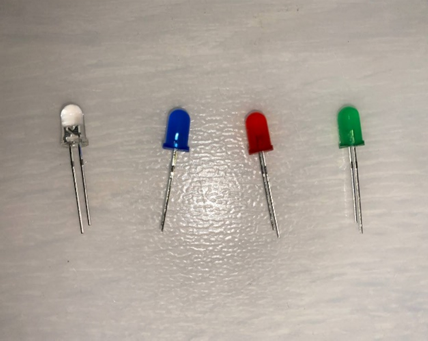
\includegraphics{image1.png}}
\caption{LED}
\label{fig}
\end{figure}

\begin{figure}[htbp]
\centerline{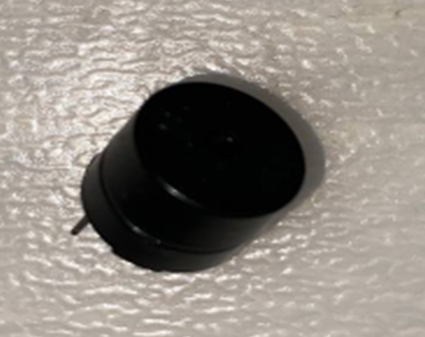
\includegraphics{image2.png}}
\caption{LED}
\label{fig}
\end{figure}

\begin{figure}[htbp]
\centerline{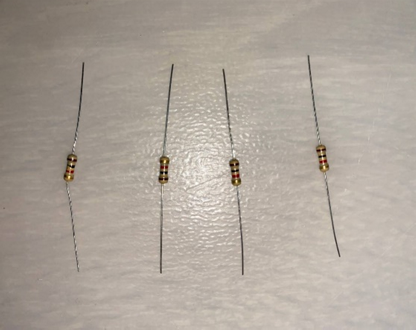
\includegraphics{image3.png}}
\caption{LED}
\label{fig}
\end{figure}

\begin{figure}[htbp]
\centerline{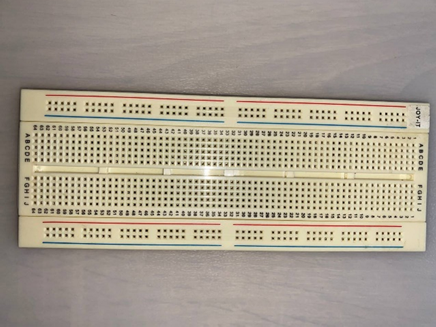
\includegraphics{image4.png}}
\caption{LED}
\label{fig}
\end{figure}

\begin{figure}[htbp]
\centerline{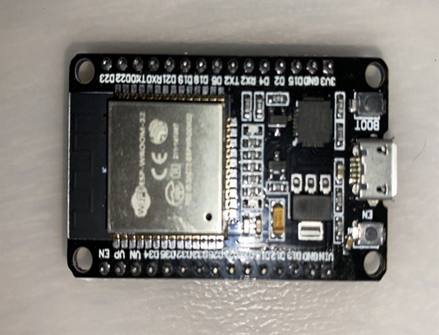
\includegraphics{image5.png}}
\caption{LED}
\label{fig}
\end{figure}





\begin{table}[]
\begin{center}
\caption{Features in Smart Light}
\begin{tabular}{|l|l|}
\hline
No & Smart   Light Features \\ \hline
2. & Turn on LED            \\ \hline
3. & Turn off LED           \\ \hline
4. & Turn on night mode     \\ \hline
5. & Turn on party mode     \\ \hline
6. & Change color           \\ \hline
7. & Play sound             \\ \hline
\end{tabular}
\end{center}
\end{table}






\begin{table}[]
\begin{center}
\caption{Lists of commands}
\begin{tabular}{|l|l|}
\hline
List of Commands & Function             \\ \hline
ONW              & Turn on white LED    \\ \hline
ONR              & Turn on red LED      \\ \hline
ONB              & Turn on blue LED     \\ \hline
ONG              & Turn on green LED    \\ \hline
OFFW             & Turn off white LED   \\ \hline
OFFR             & Turn off red LED     \\ \hline
OFFB             & Turn off blue LED    \\ \hline
OFFG             & Turn off green LED   \\ \hline
BLW              & Blinking white LED   \\ \hline
BLR              & Blinking red LED     \\ \hline
BLB              & Blinking blue LED    \\ \hline
BLG              & Blinking green LED   \\ \hline
NMW              & Night mode white LED \\ \hline
NMR              & Night mode red LED   \\ \hline
NMB              & Night mode blue LED  \\ \hline
NMG              & Night mode green LED \\ \hline
PARTY            & Party mode           \\ \hline
\end{tabular}
\end{center}
\end{table}


\begin{figure}[htbp]
\centerline{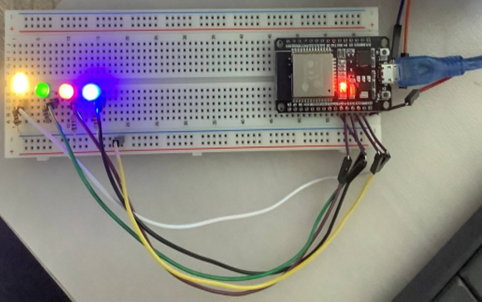
\includegraphics{image7.png}}
\caption{LED}
\label{fig}
\end{figure}




\begin{figure}[htbp]
\centerline{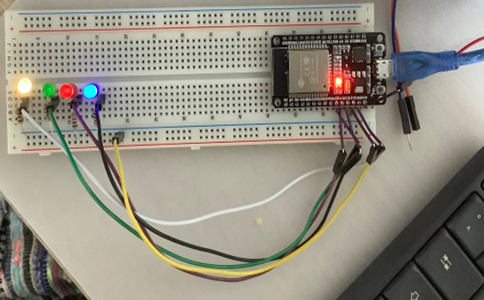
\includegraphics{image8.png}}
\caption{LED}
\label{fig}
\end{figure}


\begin{figure}[htbp]
\centerline{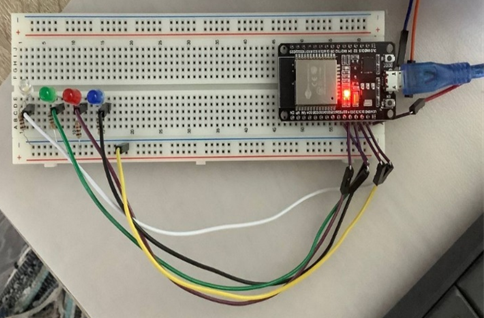
\includegraphics{image9.png}}
\caption{LED}
\label{fig}
\end{figure}



\begin{figure}[htbp]
\centerline{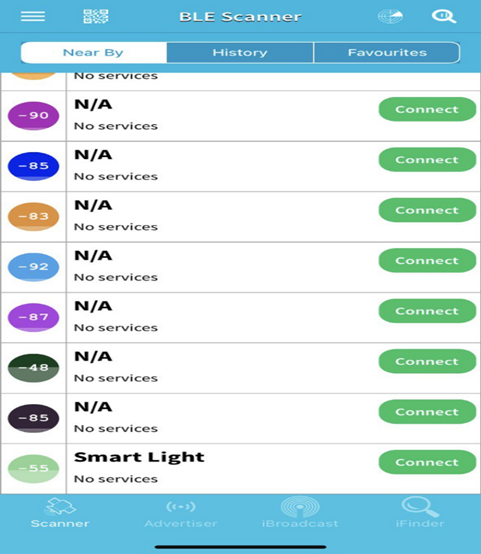
\includegraphics{image10.png}}
\caption{LED}
\label{fig}
\end{figure}




\begin{figure}[htbp]
\centerline{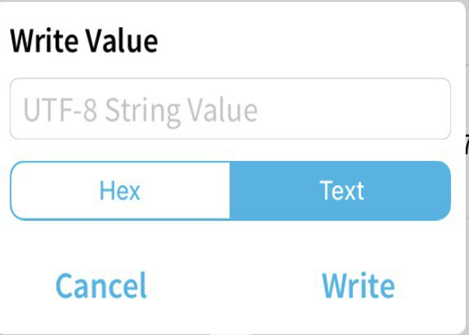
\includegraphics{image11.png}}
\caption{LED}
\label{fig}
\end{figure}








\end{document}
\section{Conclusion}

ösdaboöbvsabölva,mvböao



\end{document}
